%\documentclass[landscape,a0b,final,a4resizeable]{a0poster}
%\documentclass[landscape,a0b,final]{a0poster}
%\documentclass[portrait,a0b,final,a4resizeable]{a0poster}
\documentclass[portrait,a0b,final]{a0poster}
%%% Option "a4resizeable" makes it possible ot resize the
%   poster by the command: psresize -pa4 poster.ps poster-a4.ps
%   For final printing, please remove option "a4resizeable" !!

\usepackage{epsfig}\usepackage{multicol}
\usepackage{pstricks,pst-grad}
\usepackage{calc,amsmath}
\usepackage[dcucite]{harvard}
\usepackage{epsfig,psfrag}

%%%%%%%%%%%%%%%%%%%%%%%%%%%%%%%%%%%%%%%%%%%
% Definition of some variables and colors
%\renewcommand{\rho}{\varrho}
%\renewcommand{\phi}{\varphi}
\setlength{\columnsep}{3cm}
\setlength{\columnseprule}{2mm}
\setlength{\parindent}{0.0cm}



%%%%%%%%%%%%%%%%%%%%%%%%%%%%%%%%%%%%%%%%%%%%%%%%%%%%
%%%               Background                     %%%
%%%%%%%%%%%%%%%%%%%%%%%%%%%%%%%%%%%%%%%%%%%%%%%%%%%%

\newcommand{\background}[3]{
  \newrgbcolor{cgradbegin}{#1}
  \newrgbcolor{cgradend}{#2}
  \psframe[fillstyle=gradient,gradend=cgradend,
  gradbegin=cgradbegin,gradmidpoint=#3](0.,0.)(1.\textwidth,-1.\textheight)
}

%%%%%%%
% Enormous fint size
%%%%%%

\newcommand{\Enormous}[0]{\fontsize{3.0cm}{2.5cm}\selectfont}

%%%%%%%%%%%%%%%%%%%%%%%%%%%%%%%%%%%%%%%%%%%%%%%%%%%%
%%%                Poster                        %%%
%%%%%%%%%%%%%%%%%%%%%%%%%%%%%%%%%%%%%%%%%%%%%%%%%%%%
\newenvironment{poster}{
  \begin{center}
  \begin{minipage}[c]{0.98\textwidth}
}{
  \end{minipage} 
  \end{center}
}



%%%%%%%%%%%%%%%%%%%%%%%%%%%%%%%%%%%%%%%%%%%%%%%%%%%%
%%%                pcolumn                       %%%
%%%%%%%%%%%%%%%%%%%%%%%%%%%%%%%%%%%%%%%%%%%%%%%%%%%%

\newenvironment{pcolumn}[1]{
  \begin{minipage}{#1\textwidth}
  \begin{center}
}{
  \end{center}
  \end{minipage}
}



%%%%%%%%%%%%%%%%%%%%%%%%%%%%%%%%%%%%%%%%%%%%%%%%%%%%
%%%                pbox                          %%%
%%%%%%%%%%%%%%%%%%%%%%%%%%%%%%%%%%%%%%%%%%%%%%%%%%%%

\newrgbcolor{lcolor}{0. 0. 0.80}
\newrgbcolor{gcolor1}{1. 1. 1.}
\newrgbcolor{gcolor2}{.80 .80 1.}

\newcommand{\pbox}[4]{
\psshadowbox[#3]{
\begin{minipage}[t][#2][t]{#1}
#4
\end{minipage}
}}



%%%%%%%%%%%%%%%%%%%%%%%%%%%%%%%%%%%%%%%%%%%%%%%%%%%%
%%%                myfig                         %%%
%%%%%%%%%%%%%%%%%%%%%%%%%%%%%%%%%%%%%%%%%%%%%%%%%%%%
% \myfig - replacement for \figure
% necessary, since in multicol-environment 
% \figure won't work

\newcommand{\myfig}[3][0]{
\begin{center}
  \vspace{1.5cm}
  \includegraphics[width=#3\hsize,angle=#1]{#2}
  \nobreak\medskip
\end{center}}



%%%%%%%%%%%%%%%%%%%%%%%%%%%%%%%%%%%%%%%%%%%%%%%%%%%%
%%%                mycaption                     %%%
%%%%%%%%%%%%%%%%%%%%%%%%%%%%%%%%%%%%%%%%%%%%%%%%%%%%
% \mycaption - replacement for \caption
% necessary, since in multicol-environment \figure and
% therefore \caption won't work

%\newcounter{figure}
\setcounter{figure}{1}
\newcommand{\mycaption}[1]{
  \vspace{0.1cm}
  \begin{quote}
    {{\sc Figure} \arabic{figure}: #1}
  \end{quote}
  \vspace{0.5cm}
  \stepcounter{figure}
}


%%%%%%%%%%%%%%%%%%%%%%%%%%%%%%%%%%%%%%%%%%%%%%%%%%%%
%%%                some definitions              %%%
%%%%%%%%%%%%%%%%%%%%%%%%%%%%%%%%%%%%%%%%%%%%%%%%%%%%
\newcommand{\ca}{\mathcal{A}}
\newcommand{\vc}[1]{\mbox{\boldmath $#1$}}

%%%%%%%%%%%%%%%%%%%%%%%%%%%%%%%%%%%%%%%%%%%%%%%%%%%%%%%%%%%%%%%%%%%%%%
%%% Begin of Document
%%%%%%%%%%%%%%%%%%%%%%%%%%%%%%%%%%%%%%%%%%%%%%%%%%%%%%%%%%%%%%%%%%%%%%

\begin{document}


%\vspace*{1cm}


\newrgbcolor{lightblue}{0. 0. 0.80}
\newrgbcolor{white}{1. 1. 1.}
\newrgbcolor{whiteblue}{.80 .80 1.}
\newrgbcolor{NTNUblue}{0.0039 0.0469 0.5273}

%\background{1. 1. 1.}{1. 1. 1.}{0.5}
\background{.8 .8 1.}{1. 1. 1.}{0.5}
\def\mm#1{\ensuremath{\boldsymbol{#1}}} % version: amsmath

\begin{poster}

%%%%%%%%%%%%%%%%%%%%%
%%% Header
%%%%%%%%%%%%%%%%%%%%%
\begin{center}
\begin{pcolumn}{0.98}

\pbox{0.95\textwidth}{}{shadowsize=30pt,linewidth=2mm,framearc=0.3,linecolor=NTNUblue,fillstyle=gradient,gradangle=0,gradbegin=white,gradend=whiteblue,gradmidpoint=1.0,framesep=1em}{

%%% Unisiegel
\begin{minipage}[c][15cm][c]{0.15\textwidth}
  \begin{center}
    
\includegraphics[width=11cm,angle=0]{ntnulogo5.eps}
  \end{center}
\end{minipage}
%%% Titel
\begin{minipage}[c][16cm][c]{0.85\textwidth}
  \begin{center}
    {\bf \Enormous  Isogeometric finite element analysis - integrating design and analysis }\\[10mm]

    {\Huge Kjetil Andr\'e Johannessen\\[7.5mm]
        Norwegian University of Science and Technology, Trondheim, Norway}
\end{center}
\end{minipage}
}
\end{pcolumn}
\end{center}

\vspace*{1.5cm}

%%%%%%%%%%%%%%%%%%%%%
%%% Content
%%%%%%%%%%%%%%%%%%%%%
\begin{multicols}{3}
    \vspace{1cm}
    \pbox{\columnwidth-\columnsep}{13.9cm}{linewidth=2mm,framearc=0.1,linecolor=whiteblue,fillstyle=gradient,gradangle=0,gradbegin=white,gradend=white,gradmidpoint=1.0,framesep=1em,shadowsize=10pt}{
        \Large{{\bf Abstract:} By using splines as a basis for finite element computations,
		we get the benifit of both high order functions and smooth functions.
		Moreover, B-splines and NURBS is the dominant technology in commercial CAD systems,
		which makes it possible to keep the same model representation from design,
		to analysis to visualization through the entire production pipeline. }
    }
    \vspace{1cm}
    \begin{center}{\huge{\bf Design}}
    \end{center}
    \vspace{1cm}
    % \setlength{\columnseprule}{0pt}
    % \begin{multicols}{2}
    \Large{\bf Basis functions}
		Given a knot vector of nondecreasing knots $\Xi=[\xi_1, \xi_2, \xi_3, ... \xi_{n+p+1}]$ we define the set of $n$ basisis functions by

    	\pbox{\columnwidth-\columnsep}{10.2cm}{linewidth=2mm,framearc=0.1,linecolor=whiteblue,fillstyle=gradient,gradangle=0,gradbegin=whiteblue,gradend=whiteblue,gradmidpoint=1.0,framesep=1em,shadowsize=10pt}{
			\begin{equation}
				\label{eq:bspline}
				N_{i,p}(\xi) = \frac{\xi - \xi_i}{\xi_{i+p}-\xi_i}N_{i,p-1}(\xi) + \frac{\xi_{i+p+1}-\xi}{\xi_{i+p+1}-\xi_{i+1}}N_{i+1,p-1}(\xi),
			\end{equation}
			and,
			\begin{equation*}
				\label{eq:bspline-start}
				N_{i,0}(\xi) = \left\{
				\begin{array}{ll}
					1	&	$if $ \ \ \xi \in [\xi_i, \xi_{i+1}) \\
					0	&	$else$
				\end{array}
				\right.
			\end{equation*}
		}
		where $p$ is the polynomial degree. These functions are piecewise polynomial and smooth at the knot values themselves. \\
		\begin{center}
			\epsfig{file=bspline-set.eps,width=16cm,angle=0} \\
			\normalsize{Fig 1: The set of quadratic basis functions to the knot vector $\Xi=[0,0,0,1,2,3,3,4,4,4]$}
		\end{center}

		\vspace{0.5cm}

		By weighting each basis function with a control point, we are able to create curves
		\begin{equation*}
			\mathbf{f}(\xi) = \sum_{i=1}^n \mathbf{B}_i N_{i,p}(\xi)
		\end{equation*}

		\vspace{1cm}
		
		\begin{center}
			\epsfig{file=curves.eps,width=13cm,angle=0}  \\
			\normalsize{Fig 2: A B-spline curve given by its controlpoints $\mathbf{B}_i$}
		\end{center}
		
        
    % \end{multicols}
	\vspace{1cm}
    \Large{\bf Bi- and trivariate Splines}
		By creating a tensor product of two or three univariate splines, we are able to create surface and solid representations, i.e. 
		\begin{equation*}
			\mathbf{F}(\xi,\eta) = \sum_{i=1}^n \sum_{j=1}^n \mathbf{B}_{i,j} N_{i,p}(\xi)N_{j,q}(\eta)
		\end{equation*}
		for bivariate surfaces. This allows us to generate mappings from the reference coordinates $(\xi,\eta,\zeta)$ which forms a regular rectangle or box into a complex geometry in physical space given by $(x,y,z)$-coordinates.
		\begin{center}
			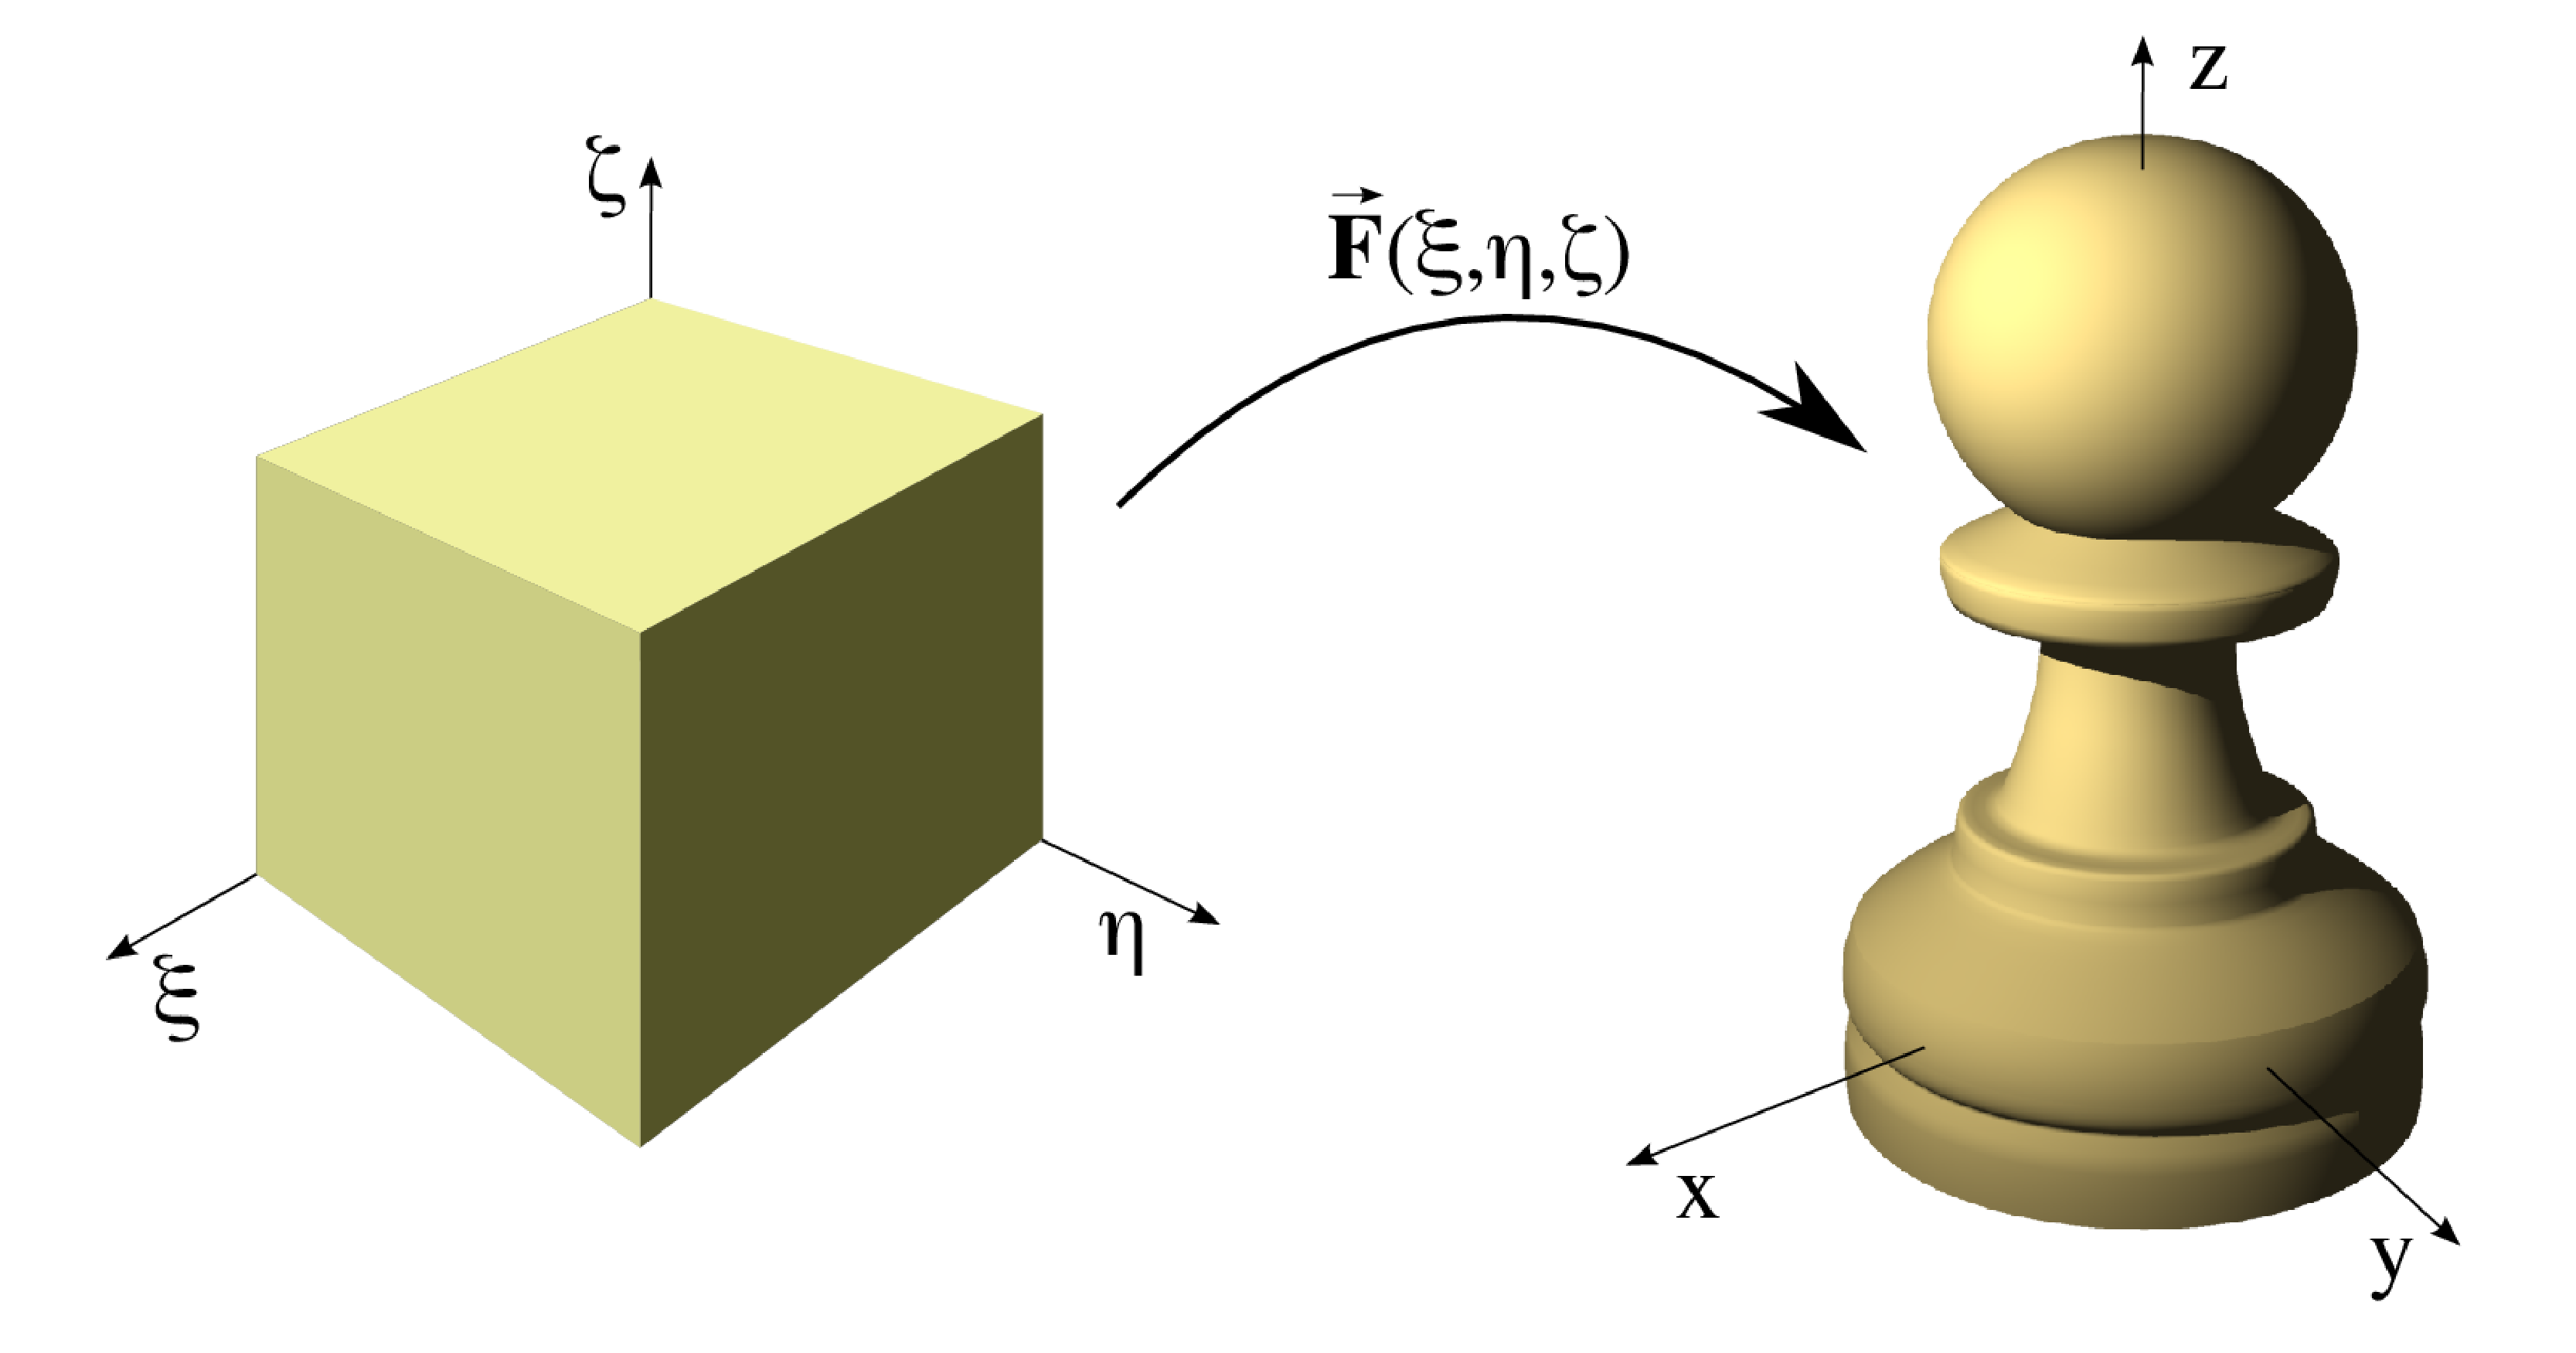
\epsfig{file=pawn-mapping.eps,width=16cm,angle=0} 
			
\epsfig{file=MappingQR.eps,height=5cm,angle=0} \\
			\normalsize{Fig 3: A trivariate NURBS solid mapping}
		\end{center}

    \vspace{1cm}

    \pbox{\columnwidth-\columnsep}{16.5cm}{linewidth=2mm,framearc=0.1,linecolor=NTNUblue,fillstyle=gradient,gradangle=0,gradbegin=white,gradend=white,gradmidpoint=1.0,framesep=1em,shadowsize=10pt}{
        {\bf Mesh generation:}
		The mesh is generated in a commercial CAD program (Rhino) and transfered to our finite element analysis
		code \emph{without any loss} in accuracy. It is using the same representation in both design and
		analysis. \\
		\epsfig{file=rhino.eps,width=13cm,angle=0} 
		\epsfig{file=RhinoQR.eps,height=5cm,angle=0} 
	}

	\vspace{2cm}

    \begin{center}{\huge{\bf Analysis}}
    \end{center}
	\Large
	{\bf Differential equation}
	We emphasize the fact that this is general finite element method and any is not limited to particular differential equations. Here we have chosen the following \\
   	\pbox{\columnwidth-\columnsep}{5.2cm}{linewidth=2mm,framearc=0.1,linecolor=whiteblue,fillstyle=gradient,gradangle=0,gradbegin=whiteblue,gradend=whiteblue,gradmidpoint=1.0,framesep=1em,shadowsize=10pt}{
		{\bf Model problem} Free vibration
		\[
			\rho \frac{\partial^2 \mathbf{u}}{\partial t^2} = \nabla \sigma (\mathbf{u})
		\]
	}
	\newline

	\vspace{2cm}

	{\bf Finite element discretization} By multiplying with a test function and integrating over our domain we arrive at the linear system of equations
	\begin{equation}
	\label{eq:linearproblem}
		M\ddot{\mathbf{u}} = A\mathbf{u}
	\end{equation}
	Notice that what is separating isogeometric analysis from more classical linear finite element analysis is the choice of basis functions, where we now choose the B-spline basis functions.
	Equation \eqref{eq:linearproblem} is then further reduced to the generalized eigenvalue problem
	\begin{equation*}
		\omega^2M{\mathbf{u}} = A\mathbf{u}
	\end{equation*}
	when you are only looking for periodic solutions of the type $u=Ce^{i\omega t}$.

	\vspace{2cm}

    \begin{center} {\huge{\bf Results}} \end{center}
	\Large
		The non-zero eigenmodes of the chess piece shown as the displaced geometry
		\begin{center}
			\epsfig{file=Pawn7.eps,height=8cm,angle=0} 
			\epsfig{file=Pawn7QR.eps,height=5cm,angle=0} \\
			\normalsize{Fig 4: The 7th eigenmode}
		\end{center}
		\begin{center}
			\epsfig{file=Pawn10.eps,height=8cm,angle=0} 
			\epsfig{file=Pawn10QR.eps,height=5cm,angle=0} \\
			\normalsize{Fig 5: The 10th eigenmode}
		\end{center}
		\begin{center}
			\epsfig{file=Pawn14.eps,height=8cm,angle=0} 
			\epsfig{file=Pawn14QR.eps,height=5cm,angle=0} \\
			\normalsize{Fig 6: The 14th eigenmode}
		\end{center}

    \begin{center} {\huge{\bf More work}} \end{center}
	\Large
	{\bf Nonlinear elasticity}
		This is the results from a nonlinear elasticity equation using isogeometric finite elements
		\begin{center}
			\epsfig{file=chess.eps,height=8cm,angle=0} 
			\epsfig{file=CapablancaQR.eps,height=5cm,angle=0} \\
			\normalsize{Fig 7: Nonlinear elasticity}
		\end{center}

	{\bf Advanced models, few degrees-of-freedom}
		This model is created using 166 unique control points and 402 degrees of freedom in the finite element analysis.
		\begin{center}
			\epsfig{file=pipe.eps,width=16cm,angle=0} \\
			\normalsize{Fig 8: Nonlinear elasticity - coarse model}
		\end{center}
		

\small{
    \bibliographystyle{unsrt}
    \bibliography{mybib}
    % \end{pcolumn}
}
\end{multicols}

\end{poster}

\end{document}

